\section{Machine learning}

Machine learning (ML) is a type of artificial intelligence (AI) that allows software applications to become more accurate in predicting outcomes without being explicitly programmed. The basic premise of machine learning is to build algorithms, very efficient, that can receive input data and use statistical analysis to predict an output value within an acceptable range.

Machine learning algorithms are often categorized as being supervised or unsupervised. Supervised algorithms require humans to provide both input and desired output, in addition to furnishing feedback about the accuracy of predictions during training. Once training is complete, the algorithm will apply what was learned to new data. Unsupervised algorithms don't need to be trained with desired outcome data. Instead, they use an iterative approach called deep learning to review data and arrive at conclusions. Unsupervised learning algorithms are used for more complex processing tasks than supervised learning systems.

\subsection{Supervised learning}

One of the main types of automatic learning is supervised learning. This type of learning is akin to human learning based on the acquisition of new knowledge and skills through the experiences of the past. That means, the computer learns from data it has previously collected.

Changing the synaptic forces is based on the comparison between the output vector $ y ^ t = (y ^ t_1, y ^ t_2, ..., y ^ t_m), t = 1, ..., P $ obtained at the output layer and the target vector $ z ^ t = (z ^ t_1, z ^ t_2, ..., z ^ t_m), t = 1, ..., P $, representing the desired result to be obtained at the output layer, at the input layer the input vector $ x ^ t = (x ^ t_0, x ^ t_1, x ^ t_2, ..., x ^ t_n), t = 1, ..., P $ of the training.

The target vector $ z ^ t $ is provided by a teacher (coach-supervisor), hence the supervised learning name. Supervised learning involves the presentation by a coach of pairs of data form $ (x ^ t, z ^ t), t = 1, ..., P $ forming a set of data, called training set: $$ S = \{(x ^ t, z ^ t) | t = 1, ..., P \} $$

The difference between the obtained y response and the desired z response is the error and is used to modify the synaptic forces, based on a specific algorithm called \cite{calculNeuronal}.

We can represent supervised learning with the following diagram \cite{Baum}:

\begin{figure}[H]
  \centering
  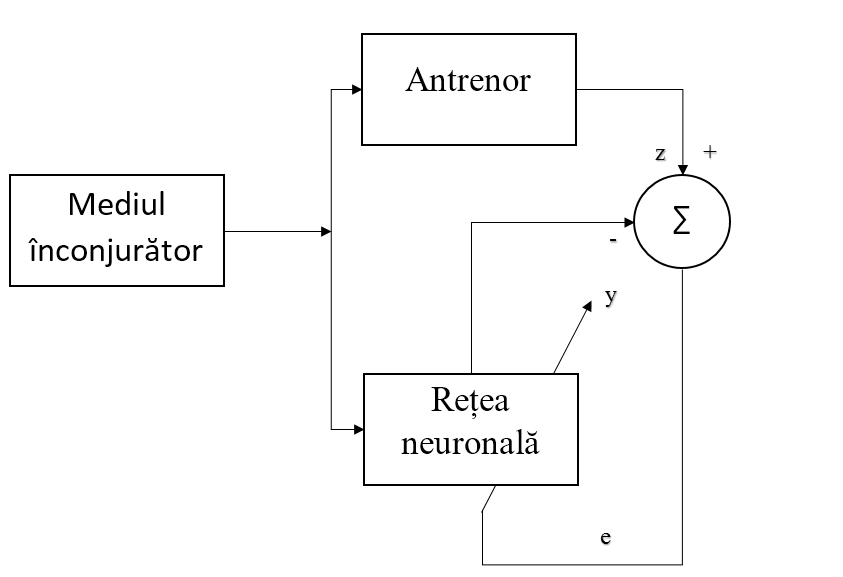
\includegraphics[width=3.5in]{images/diagramaInvSupervizate.png}
  \caption {Diagram of supervised learning.}
\end{figure}

It is seen from this diagram the equivalence of the supervised learning paradigm with the learning algorithm based on minimizing the error function \cite{Haykin}.
\subsection{Unsupervised learning}

Unsupervised learning involves learning without a coach \cite{Girolami}. The neural network must be able to "discover" patterns, features, correlations or categories in the input data set themselves and encode them in the form of output data \cite{Sanger1, Sanger2}. Neural network connections and neurons must represent a degree of self-organization.

Unsupervised learning can only be used when there is redundancy in the input data set. Without redundancy, it is impossible to discover any pattern or trait in the set of input data. From this point of view, redundancy ensures knowledge \cite{Barlow}.

The diagram below is the paradigm of unsupervised learning:

\begin{figure}[H]
  \centering
  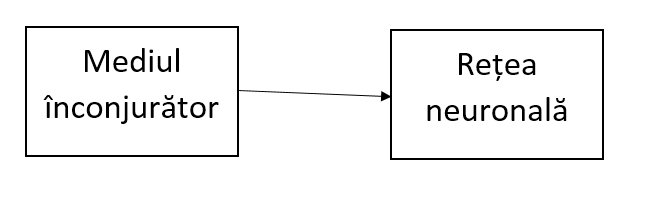
\includegraphics[width=3in]{images/diagramaInvNesupervizate.png}
  \caption {Unsupervised Learning Diagram.}
\end{figure}

In unsupervised learning, we have information about a measure of the quality of representation that the neural network needs to reach through the learning process \cite{Diamantaras}. Its parameters will be optimized for this measure. If the learning process is over, the neural network will be able to form internal representations that encode the input data features and automatically create new classes \cite{Diamantaras}.

We can use a competitive learning algorithm or a Hebbian learning algorithm for a neural network to be able to perform unsupervised learning.
\subsection{Learning optimizer}

Optimization refers to the task of minimizing/maximizing an objective function $f(x)$ parameterized by $x$. In machine/deep learning terminology, it’s the task of minimizing the cost/loss function $J(w)$ parameterized by the model’s parameters $w \in R^d$. Optimization algorithms (in case of minimization) have one of the following goals:

\begin{itemize}
    \item Find the lowest possible value of the objective function within its neighborhood. That’s usually the case if the objective function is not convex as the case in most deep learning problems.
    \item Find the global minimum of the objective function. This is feasible if the objective function is convex, i.e. any local minimum is a global minimum.
\end{itemize}

There are three kinds of optimization algorithms:

\begin{itemize}
    \item Optimization algorithm that is iterative in nature and converges to acceptable solution regardless of the parameters initialization such as gradient descent applied to logistic regression.
    \item Optimization algorithm that is iterative in nature and applied to a set of problems that have non-convex cost functions such as neural networks. Therefore, parameters’ initialization plays a critical role in speeding up convergence and achieving lower error rates.
    \item Optimization algorithm that is not iterative and simply solves for one point.
\end{itemize}

\subsubsection{Adam optimizer}

The method computes individual adaptive learning rates for different parameters from estimates of first and second moments of the gradients; the name Adam is derived from adaptive moment estimation. This is used to perform optimization and is one of the best optimizer at present. The author claims that it inherits from RMSProp and AdaGrad (Well it inherits from them).\\

Features:
\begin{itemize}
    \item The step-size is approximately bounded by the step-size hyper-parameter.
    \item It doesn't require stationary objective. That means the f(x) we talked about might change with time and still the algorithm will converge.
    \item Parameters update are invariant to re-scaling of gradient. It means that if we have some objective function f(x) and we change it to $k*f(x)$ (where k is some constant). There will be no effect on performance.
    \item Naturally performs step size annealing. Well remember the classical SGD, we used to decrease step size after some epochs, nothing as such is needed here.
\end{itemize}

The method is straightforward to implement, is computationally efficient, has little memory requirements, is invariant to diagonal rescaling of the gradients, and is well suited for problems that are large in terms of data and/or parameters \cite{Diederik}. 

\begin{algorithm}
    \SetKwInOut{Input}{Input}
    \SetKwInOut{Output}{Output}

    \Input{$\alpha$: Stepsize}
    \Input{$\beta_1, \beta_2 \in [0, 1)$: Exponential decay rates for the moment estimates}
    \Input{$f(\theta)$: Stochastic objective function with parameters $\theta$}
    \Input{$\theta_0$: nitial parameter vector}
    
    $m_0 \leftarrow 0$ (Initialize $1^{st}$ moment vector)\;
    $v_0 \leftarrow 0$ (Initialize $2^{nd}$ moment vector)\;
    $t \leftarrow 0$ (Initialize timestep)\;
    
    \While {$\theta_t$ not converged} {
        $t \leftarrow t + 1$ \;
        $g_t \leftarrow \bigtriangledown_0 f_1 (\theta_{t-1})$ (Get gradients w.r.t. stochastic objective at timestept)\;
        $m_t \leftarrow \beta_1 \cdot m_{t-1} + (1 - \beta_1) \cdot g_t$ (Update biased first moment estimate)\;
        $v_t \leftarrow \beta_2 \cdot v_{t-1} + (1-\beta_2) \cdot g_t^2$ (Update biased second raw moment estimate)\;
        $\widehat{m}_t \leftarrow m_t/(1 - \beta_1^t)$ (Compute bias-corrected first moment estimate)\;
        $\widehat{v}_t \leftarrow v_t/(1 - \beta_2^t)$ (Compute bias-corrected second raw moment estimate)\;
        $\theta_t \leftarrow \theta_{t-1} - \alpha \cdot \widehat{m}_t / (\sqrt{\widehat{v}_t} + e)$ (Update parameters)\;
    }
    
    \Return $\theta_t$ (Resulting parameters)

    \label{alg:adamOptimizer}
    \caption{Adam, proposed algorithm for stochastic optimization.}
\end{algorithm}

Let $f(\theta)$ be  a  noisy  objective  function:  a  stochastic  scalar  function  that  is  differentiable  w.r.t. parameters $\theta$. We  are  interested in minimizing the expected value of this function, $E[f(\theta)]$ w.r.t. its parameters $\theta$. With $f_1(θ),...,f_T(θ)$ we  denote  the  realisations  of  the  stochastic  function  at  subsequent  timesteps 1,...,T. The stochasticity might come from the evaluation at random subsamples (minibatches) of datapoints, or arise from inherent function noise. With $g_t= \bigtriangledown_0 f_1 (\theta_{t-1})$ we denote the gradient, i.e. the vector of partial derivatives of $f_t.w.r.t \theta$ evaluated at timestep $t$. 

The algorithm updates exponential moving averages of the gradient $(m_t)$ and the squared gradient $(v_t)$ where the hyper-parameters $β_1,β_2 \in [0,1)$ control the exponential decay rates of these moving averages. The moving averages themselves are estimates of the $2^{nd}$ raw moment (the uncentered variance) and the $1^{st}$ moment (the mean) of the gradient.   However,  these moving averages are initialized as (vectors of) 0’s, leading to moment estimates that are biased towards zero, especially during the initial timesteps, and especially when the decay rates are small (i.e. the $\beta$s are close to 1).The good news is that this initialization bias can be easily counteracted, resulting in bias-corrected estimate $\widehat{m}_t$ and $\widehat{v}_t$.

Note that the efficiency of \ref{alg:adamOptimizer} can, at the expense of clarity, be improved upon by changing the order of computation, e.g.  by replacing the last three lines in the loop with the following lines \cite{Diederik}: $$\alpha_t = \alpha \cdot \sqrt{1 - \beta_2^t}/(1 - \beta_1^t)$$ and $$\theta_y \leftarrow \theta_{t-1} - \alpha_t \cdot m_t/(\sqrt{v_t} + \widehat{e})$$


\subsubsection{AdaGrad optimizer}

AdaGrad or adaptive gradient allows the learning rate to adapt based on parameters. It performs larger updates for infrequent parameters and smaller updates for frequent one. Because of this it is well suited for sparse data (NLP or image recognition). Another advantage is that it basically eliminates the need to tune the learning rate. Each parameter has its own learning rate and due to the peculiarities of the algorithm the learning rate is monotonically decreasing. This causes the biggest problem: at some point of time the learning rate is so small that the system stops learning.

\subsubsection{Gradient descendent optimizer}

Gradient Descent is the most common optimization algorithm in machine learning and deep learning. It is a first-order optimization algorithm. This means it only takes into account the first derivative when performing the updates on the parameters. On each iteration, we update the parameters in the opposite direction of the gradient of the objective function J(w) w.r.t the parameters where the gradient gives the direction of the steepest ascent. The size of the step we take on each iteration to reach the local minimum is determined by the learning rate $\alpha$. Therefore, we follow the direction of the slope downhill until we reach a local minimum.

\subsubsection{RMSprop optimizer}

Gradients of very complex functions like neural networks have a tendency to either vanish or explode as the energy is propagated through the function. And the effect has a cumulative nature; the more complex the function is, the worse the problem becomes.

Rmsprop is a very clever way to deal with the problem. It uses a moving average of squared gradients to normalize the gradient itself. That has an effect of balancing the step size; decrease the step for large gradient to avoid exploding, and increase the step for small gradient to avoid vanishing.
\subsection{Recurrent neural network}

Humans don’t start their thinking from scratch every second. As you read this essay, you understand each word based on your understanding of previous words. You don’t throw everything away and start thinking from scratch again. Your thoughts have persistence.

Traditional neural networks can’t do this, and it seems like a major shortcoming. For example, imagine you want to classify what kind of event is happening at every point in a movie. It’s unclear how a traditional neural network could use its reasoning about previous events in the film to inform later ones.

Recurrent neural networks address this issue. They are networks with loops in them, allowing information to persist.

\begin{figure}[H]
    \centering
    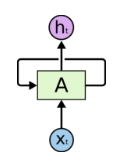
\includegraphics[width=2in]{images/rnn.png}
    \caption{Recurrent Neural Networks with loops.}
    \label{fig:rnnRoll}
\end{figure}

In the above diagram, a chunk of neural network, $A$, looks at some input $x_t$ and outputs a value $h_t$. A loop allows information to be passed from one step of the network to the next.

These loops make recurrent neural networks seem kind of mysterious. However, if you think a bit more, it turns out that they aren’t all that different than a normal neural network. A recurrent neural network can be thought of as multiple copies of the same network, each passing a message to a successor. Consider what happens if we unroll the loop:

\begin{figure}[H]
    \centering
    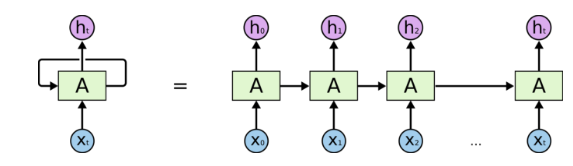
\includegraphics[width=6.5in]{images/rnnUnroll.png}
    \caption{Unrolled recurrent neural network.}
    \label{fig:rnnUnroll}
\end{figure}

This chain-like nature reveals that recurrent neural networks are intimately related to sequences and lists. For such data, they are the natural architecture of neural network.

And they certainly are used! In the last few years, there have been incredible success applying RNNs to a variety of problems: speech recognition, language modeling, translation, image captioning… The list goes on.

Over the years researchers have developed more sophisticated types of RNNs to deal with some of the shortcomings of the vanilla RNN model. I want this section to serve as a brief overview so that you are familiar with the taxonomy of models.

\subsubsection{Bidirectional RNNs}

Bidirectional recurrent neural networks(RNN) are really just putting two independent RNNs together. The input sequence is fed in normal time order for one network, and in reverse time order for another. The outputs of the two networks are usually concatenated at each time step, though there are other options, e.g. summation.

\begin{figure}[H]
    \centering
    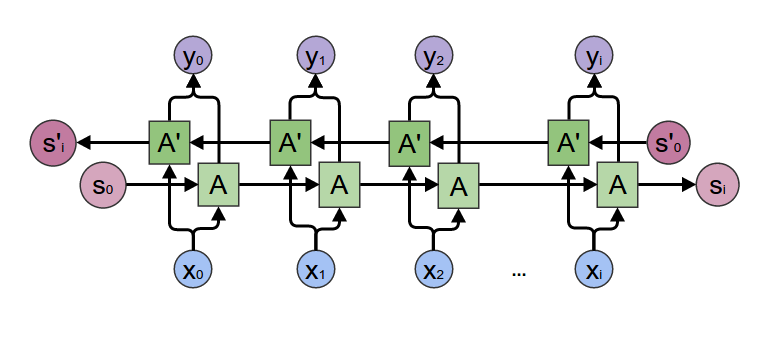
\includegraphics[width=6.5in]{images/bidirectionalRNN.png}
    \caption{General Structure of Bidirectional Recurrent Neural Networks.}
    \label{fig:bidirectionalRNN}
\end{figure}

This structure allows the networks to have both backward and forward information about the sequence at every time step.

They're often used when we’re trying to make predictions in a sequence. For example, in voice recognition, we might wish to predict a phenome for every time step in an audio segment, based on past context.

\subsubsection{Deep (Bidirectional) RNNs}

They're similar to Bidirectional RNNs, only that we now have multiple layers per time step. In practice this gives us a higher learning capacity (but we also need a lot of training data).

\subsubsection{LSTM networks}

One of the appeals of RNNs is the idea that they might be able to connect previous information to the present task. That work such as using previous video frames might inform the understanding of the present frame. If RNNs could do this, they’d be extremely useful. But can they? It depends.

Sometimes, to perform the present task, we only need to look at recent information. For example, consider a language model trying to predict the next word based on the previous ones. We don’t need any further context if we are trying to predict the last word in “the clouds are in the sky,”. – it’s pretty obvious the next word is going to be sky. In such cases, where the gap between the relevant information and the place that it’s needed is small, RNNs can learn to use the past information.


\begin{figure}[H]
    \centering
    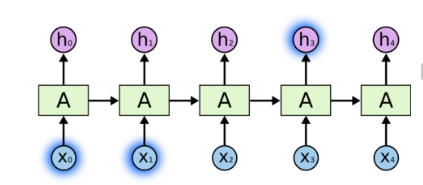
\includegraphics[width=4.5in]{images/rnnWhatWeNeed.png}
    \caption{Graphics representation for connecting informations}
\end{figure}


But there are also cases where we need more context. Consider trying to predict the last word in the text “I grew up in France… I speak fluent French.” Recent information suggests that the next word is probably the name of a language, but we need the context of France, from further back if we want to narrow down which language. It’s entirely possible for the gap between the relevant information and the point where it is needed to become very large.

Unfortunately, as that gap grows, RNNs become unable to learn to connect the information.

\begin{figure}[H]
    \centering
    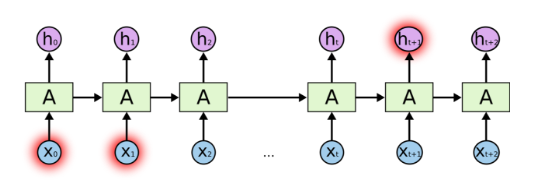
\includegraphics[width=6.5in]{images/rnnWhatWeNeedButCannot.png}
    \caption{Graphics representation for connecting informations, more data}
\end{figure}

In theory, RNNs are absolutely capable of handling such “long-term dependencies.” A human could carefully pick parameters for them to solve toy problems of this form. Sadly, in practice, RNNs don’t seem to be able to learn them. The problem was explored in depth by Hochreiter (1991) [German] and Bengio, et al. (1994), who found some pretty fundamental reasons why it might be difficult. \cite{lstm}

Thankfully, LSTMs don’t have this problem!

Long Short Term Memory networks – usually just called "LSTMs" – are a special kind of RNN, capable of learning long-term dependencies. They were introduced by Hochreiter \& Schmidhuber in 1997, and were refined and popularized by many people in following work. They work tremendously well on a large variety of problems, and are now widely used.

LSTMs are explicitly designed to avoid the long-term dependency problem. Remembering information for long periods of time is practically their default behavior, not something they struggle to learn!

All recurrent neural networks have the form of a chain of repeating modules of neural network. In standard RNNs, this repeating module will have a very simple structure, such as a single tanh layer.

\begin{figure}[H]
    \centering
    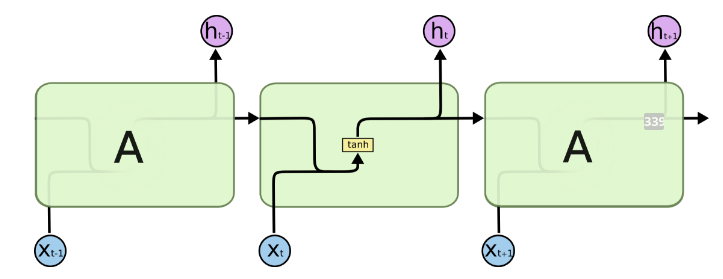
\includegraphics[width=6.5in]{images/rnnStandard.png}
    \caption{The repeating module in a standard RNN contains a single layer.}
\end{figure}

LSTMs also have this chain like structure, but the repeating module has a different structure. Instead of having a single neural network layer, there are four, interacting in a very special way.

\begin{figure}[H]
    \centering
    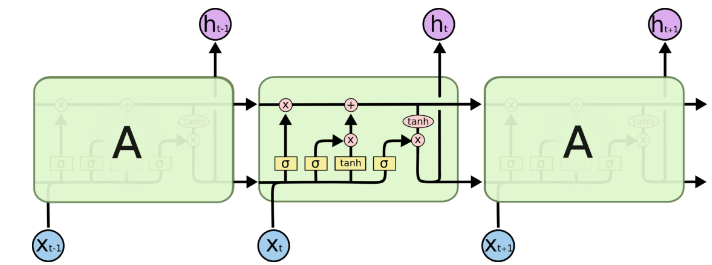
\includegraphics[width=6.5in]{images/lstm.png}
    \caption{The repeating module in an LSTM contains four interacting layers.}
\end{figure}

\subsection{Conditional random field}

Conditional Random Fields is a discriminative undirected probabilistic graphical model, a sort of Markov random field. The most often used for NLP version of CRF is linear chain CRF. CRF is a supervised learning method.

Linear chain CRF is good for different segmentation and sequence tagging tasks:

\begin{itemize}
    \item Keywords extraction
    \item (Named) Entity Recognition
    \item Sentiment Analysis
    \item Part-of-Speech Tagging
    \item Speech Recognition
\end{itemize}

The time complexity of the training process is large enough.
\begin{equation*} O(mNTQ2nS) \end{equation*}
, where:
\begin{itemize}
    \item m is the number of training iterations\
    \item N is the number of training data sequences
    \item T is the average length of training sequences
    \item Q is the number of class labels
    \item n is the number of CRF features
    \item S is the searching time of the optimization algorithm (for example, L-BFGS algorithm, which is considered good for this).
\end{itemize}

In practical implementation, the computational time is often larger due to many other operations like numerical scaling, smoothing etc. The time complexity of the inference process is much better in case of using Viterbi algorithm for inference:
\begin{equation*} О(T|S|^3) \end{equation*}
, where:

\begin{itemize}
    \item T is the number of training data sequences
    \item S is the number of class labels
\end{itemize}

The most similar method for CRF is MEMM (Maximum-entropy Markov Model). It is also discriminative probabilistic graphical model. However, MEMM has so called “label bias problem”. CRF has no such problem and this fact is the main difference between CRF and MEMM. It is not correct to compare CRF and HMM in direct way, because both CRF and HMM relate to different classes of algorithms – HMM is generative model and CRF is discriminative model.

The most evident disadvantage of CRF is high computational complexity of the training stage of the algorithm. This fact makes it more difficult to re-train the model when new training data samples become available. CRF does not work with unknown words, i.e. with words that were not present in training data sample.

Many researches show that CRF is better for NER task than MEMM and HMM. That is why Stanford NER is based on CRF. It is possible to reach high quality of labeling (e.g. for NER task) if you choose right features
CRF is flexible enough in terms of feature selection. In addition, it is not necessary for features to be conditionally independent.

\subsubsection{Keyword extraction}

As CRF is supervised machine learning algorithm, you need to have large enough training sample to train it. If you have such sample, and if you choose features wisely, theoretically you may obtain the quality around 0.6-0.7 (F1-measure)

Unfortunately, researches show us that in reality it is hardly unlikely to have a quality higher than 0.5 (F1-measure). For example, some Indian researchers used CRF to extract key words from medical texts and they had good features and large enough training sample, but they obtained quality not more than 0.4 (F1-measure). That’s sad.


\subsubsection{Named entity extraction}

CRF is significantly better in coping with NER task

For example, researchers from HSE and SPSU presented a paper, where they obtained quality of NER about 0.9 (F-measure) on a test set, having a training set not more than 70 000 examples. On real data they would hardly obtain such quality, while Stanford NER shows quality not more than 0.81 (F-measure) given it has perfectly selected training features and it was trained on larger corpora (CoNLL, MUC-6, MUC-7 and ACE)

Some Spanish and Russian researchers compared HMM and CRF in NER task for medical texts on JNLPBA corpus (18546 sentences with 109588 named entities). They obtained interesting results: HMM had higher recall (+4-7\% depending on the type of entity) while CRF had higher precision (+4-13\% depending on the type of entity). Average F-measure on cross-validation appeared to be about 0.65 for HMM and 0.69 for CRF. The authors supposed, that the quality of NER could have been 5-10\% higher if they used hybrid HMM+CRF algorithm.


\subsubsection{Time expressions extraction}

Time expressions are also entities, but very specific ones, so I decided to write about them in a separate section.

According to one master thesis, linear-chain CRF operated very well on extracting time expressions from Russian text. The author manually tagged 2000 sentences (which contained about 500 time expressions) then iteratively tuned parameters and features until he obtained 0.93 (F1-measure) in cross-validation.

Sounds cool, but in real process I think there would be no more than 0.7-0.75 (F1-measure). That is also very decent, though.

\subsubsection{Sentiment Analysis}

CRF copes with this task very well. Different research papers claim the results of using CRF for sentiment analysis for various languages are good enough – about 0.7 (F1-measure).

For instance, the researchers from HSE claimed that they achieved 0.74 (F1-measure) while performing Sentiment Analysis on real Twitter messages. They manually tagged 20 000 messages and achieved average 0.86 (F1-measure) on all three possible types of sentiment (positive, negative and neutral).

By the way, neutral class is important for a good sentiment analysis.


CRF is not very good for keywords extraction as soon as it cannot handle unknown words. Moreover, adding new data to the training dataset forcers us to re-train the whole CRF model – and it may be quite time-consuming due to the high complexity of the training phase of the algorithm.

CRF shows good performance when dealing with entity recognition (any types of entities, including named entities, time expressions, etc.). It can use both linguistic (characters, words) and non-linguistic information (upper/lower case, punctuation marks, spaces etc.). The achievable quality of entity recognition is about 0.7-0.85 (F1-measure), which is high.

There is an interesting idea to make a hybrid algorithm by combining HMM and CRF for entity recognition. Theoretically, such algorithm could increase overall quality of entity recognition by 5-10% and reach 0.85-0.9.